\section{The background channels}
The dominant SM backgrounds can be divided into two categories: (i) from leptonic $\tau$ decays and (ii) from fake leptons. In the first category, the dominant process is the pair production of $W Z$ with $W$ decaying leptonically and $Z \rightarrow \tau \tau$. The trilepton final states with no-OSSF pairs can arise from the subsequent leptonic decay of $\tau$ 's. We estimate this background process via Monte Carlo simulations.
\\
The dominant processes of the second category are $\gamma^{*} / Z+$ jets and $t \bar{t}$, where two leptons come from $\gamma^{*} / Z \rightarrow \tau \tau$ or the prompt decay of $t$ and $\bar{t}$, and a third lepton is faked from jets containing heavy-flavor mesons.
\begin{figure}
    \makebox[0.75\linewidth][c]{%
    \centering
    \begin{subfigure}{.2\textwidth}
        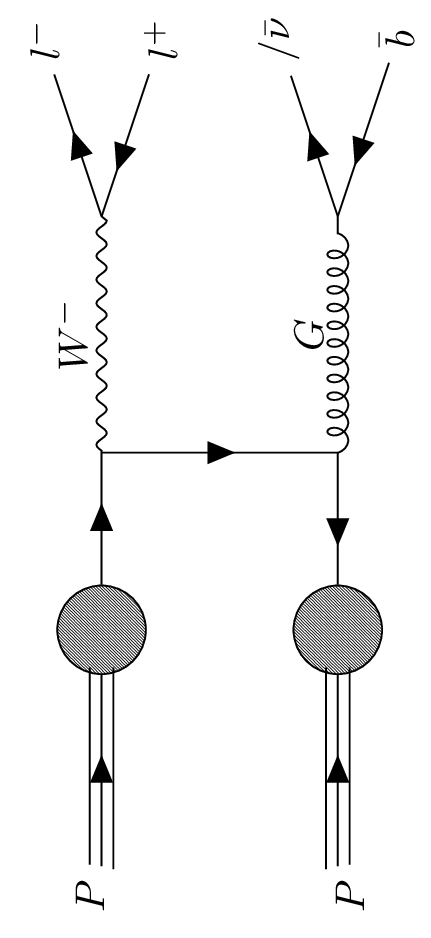
\includegraphics[width=\textwidth, angle = -90]{Figures/w_pjets.png}
        \caption{}
        \label{fig:w_pjets}
    \end{subfigure}
    \hfill
    \begin{subfigure}{.2\textwidth}
        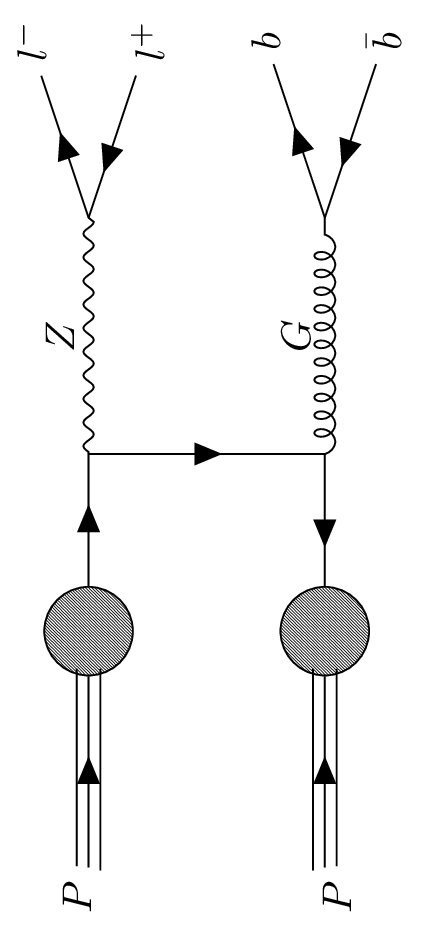
\includegraphics[width=\textwidth, angle = -90]{Figures/Z_pjets.png}
        \caption{}
        \label{fig:z_pjets}
    \end{subfigure}
    }
    \caption{}
\end{figure}